
\documentclass[]{friggeri-cv}
\usepackage{afterpage}
\usepackage{hyperref}
\usepackage{color}
\usepackage{xcolor}
\hypersetup{
    pdftitle={},
    pdfauthor={},
    pdfsubject={},
    pdfkeywords={},
    colorlinks=false,       % no lik border color
   allbordercolors=white    % white border color for all
}
\addbibresource{bibliography.bib}
\RequirePackage{xcolor}
\definecolor{pblue}{HTML}{0395DE}

\begin{document}

\header 
{\hspace{2\baselineskip} Christian C} { Lenis M}
  
% Fake text to add separator      
\fcolorbox{white}{gray}{\parbox{\dimexpr\textwidth-2\fboxsep-2\fboxrule}{%
.....
}}

% In the aside, each new line forces a line break
\begin{aside}

\includegraphics[scale=0.2]{img/Photo.png}
  \section{Datos}
    CC:1015397219
    Nacimiento:12/12/1986
    ~
  \section{Ciudad de residencia}
    Floridablanca,
    Santander
    ~
  \section{Tel }
    +57 3185712885  
    ~
  \section{Mail}
    \href{mailto:niscri@gmail.com}{\textbf{niscri@}gmail.com}
    ~
  \section{Web}
    \href{url}{{www.linkedin.com/in/}\\{christian-lenis-5692a238/}}
    ~
  \section{Habilidades}
    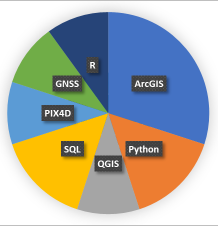
\includegraphics[scale=0.62]{img/programming.png}
   ~
  \section{Idiomas}
    \textbf{Inglés}
\includegraphics[scale=0.40]{img/3stars.png}
    \textbf{Portugués}
\includegraphics[scale=0.40]{img/3stars.png}
    \textbf{Francés}
\includegraphics[scale=0.40]{img/2stars.png}
    ~
\end{aside}

\section{Perfil}
\begin{entrylist}

  \entry
    {  }
    {Profesional analista de datos GIS\vspace{\baselineskip}}
    { }
    {\emph{Ingeniero Catastral y Geodesta, especialista en sistemas de información geográfica. Experiencia en bases de datos geográficas, análisis de datos, control de calidad cartográfica, levantamiento de información geográfica con RPAS y equipos GNSS.
    \\Conocimientos en ArcGIS, R, Python, QGIS, SQL, Pix4D, prosesamiento GNSS
}}
  
\end{entrylist}
\section{Educación}
\begin{entrylist}
  \entry
    
    {Diploma in Geographic Information Systems (Akademischer Geoinformatiker)}
    {Universität Salzburg, Salzburg Austria}
    {Especialista en sistemas de información geográfica con formación para el de diseño, desarrollo e implementación de proyectos de Geoinformación y GIS.\\}
\end{entrylist}

\begin{entrylist}
  \entry
    
    {Ingeniero Catastral y geodesta}
    {Universidad Distrital Francisco José De Caldas, Bogotá Colombia}
    {La Ingeniería Catastral y Geodesia tiene como objetivo el estudio del recurso tierra con énfasis en el manejo social como fuente generadora de bienestar, utilizando las ciencias básicas, métodos de ingeniería y ciencias de la tierra en forma Integral, apoyado del conocimiento científico e investigativo así como de técnicas y tecnologías especializadas en la medición y representación gráfica.\\}
\end{entrylist}

\section{Experiencia}
\begin{entrylist}
  \entry
    
    {Coordinador área de cartografía en Metrogas S.A. E.S.P.}
    {Floridablanca, Santander Colombia, febrero 2020 a la fecha}
    {Coordinar equipo de trabajo de cartografía para el generación de informes, análisis, almacemaniento y visualización de información cartográfica de los activos de red, usuarios y clientes potenciales de la compañía a travéz de plataformas ESRI y herramientas de gestión y análisis de datos.\\}
\end{entrylist}

\begin{entrylist}
  \entry
    
    {Ingeniero de sistemas de información georreferenciados, piloto de aeronaves no tripuladas en Ecovalor S.A.S., Rúa Abogados y Consultores}
    {Floridablanca, Santander Colombia, febrero 2018 a febrero de 2020 }
    {Procesamiento análisis y generación de información geoespacial, geográfica, gestión predial y manejo de vehículos aéreos no tripulados (vant) o dron, levantamientos GNSS, entre otras.\\}
\end{entrylist}

\begin{entrylist}
  \entry
    
    {Ingeniero Catastral y Geodesta, Control Calidad Digital SIG en  Instituto Geográfico Agustín Codazzi IGAC}
    {Bucaramanga, Santander Colombia, Octubre 2017 a noviembre de 2018 }
    {Prestación de servicios profesionales para realizar actividades de control y aprobación a la calidad de la digitalización producto de la actualización de la formación catastral del municipio de Bucaramanga, realizada por el personal contratado por el municipio.\\}
\end{entrylist}

\begin{entrylist}
  \entry
    
    {Ingeniero Catastral y Geodesta, Piloto Certificado de Dron en ENERGIZANDO S.A.S.}
    {Medellín, Antioquia Colombia, Junio 2017 a noviembre 2018}
    {Generación de ortofotografías, procesamiento fotogramétrico de imágenes generadas con RPAS, pilotaje de aeronaves no tripuladas.\\}
\end{entrylist}

\begin{entrylist}
  \entry
    
    {Ingeniero de Sistemas de información Geográfica en 3DStudio Web----}
    {Bogotá, Colombia, Febrero de 2017 a agosto de 2017}
    {Configuración, diseño, implementación y mantenimiento de bases de datos geográficas. Creación, configuración y consumo de servicios web geográficos, Procesamiento de información digital cartográfica.\\}
\end{entrylist}

\begin{entrylist}
  \entry
    
    {Ingeniero de Sistemas de información Geográfica en 3DStudio Web--}
    {Bogotá, Colombia, Enero de 2016 a diciembre de 2016}
    {Mantenimiento y actualización del sistema web de consulta de información geográfica del Ejército de la República de Colombia. Configuración, diseño, implementación y mantenimiento de bases de datos geográficas. Creación, configuración y consumo de servicios web geográficos, Procesamiento de información digital cartográfica.\\}
\end{entrylist}

\begin{entrylist}
  \entry
    
    {Auxiliar de Sistemas de información Geográfica en Arce Rojas Consultores}
    {Bogotá, Colombia, Agosto 2015 a diciembre 2015}
    {Generar lista de planchas IGAC necesarias para el proyecto de acuerdo a diseños generados. Consulta de información cartográfica existente. Elaboración de reporte de información cartográfica existente y faltante para la gestión de predios afectados por el proyecto. Recepción y archivo de documentos. Gestión documental del expediente físico. Estructuración de la información Cartográfica del proyecto. Gestión predial y cartografía para proyecto Ecopetrol de Hidrocarburos no convencionales.\\}
\end{entrylist}

\begin{entrylist}
  \entry
    
    {Técnico de Sistemas de información Geográfica en Zofre SLP Sucursal Colombia}
    {Bogotá, Colombia, Agosto 2014 a agosto 2015}
    {Gestión de datos geográficos y generación de planos para proyectos de ingeniería civil, geología y geotécnia. Elaboración de cartografía estudios geológicos y geotécnicos para el proyecto Doble Calzada Duitama Cúcuta.\\}
\end{entrylist}

\newpage

\section{Certificaciones}
\begin{entrylist}

  \entry
   {2019}
    {Curso de Ingeniería de Datos con Python}
    {Platzi}
    {\emph{https://platzi.com/p/cclenism/curso/1385-ingenieria-datos/diploma/detalle/}}
     \entry
  {2020}
    {Curso de Inteligencia Artificial con IBM Watson}
    {Platzi}
    {\emph{https://platzi.com/p/cclenism/curso/1804-ibm-watson/diploma/detalle/}}
     \entry
   {2020}
    {Curso de Machine Learning Aplicado con Python}
    {Platzi}
    {\emph{https://platzi.com/p/cclenism/curso/1178-scikit/diploma/detalle/}}
     \entry
    {2020}
    {Curso de Fundamentos Matemáticos para Inteligencia Artificial}
    {Platzi}
    {\emph{https://platzi.com/p/cclenism/curso/1729-matematicas-ai/diploma/detalle/}}
     \entry
    {2019}
    {Curso de Python}
    {Platzi}
    {\emph{https://platzi.com/p/cclenism/curso/1104-python-2019/diploma/detalle/}}
     \entry
    {2019}
    {Python Scripting for Geoprocessing Workflows}
    {Esri}
    {\emph{www.esri.com/training/TrainingRecord/Certificate/}\\{cclenism/5b32b185d54ead38aa9944b2/300}}
    \entry
    {2019}
    {Python Scripting for Map Automation}
    {Esri}
    {\emph{www.esri.com/training/TrainingRecord/Certificate/}\\{cclenism/5c7c929465e21d6e218ec0b5/300}}
    \entry
    {2018}
    {Integrating Data in ArcGIS Pro}
    {Esri}
    {\emph{www.esri.com/training/TrainingRecord/Certificate/}\\{cclenism/5b1f4aef5681d409adf037e7/300}}
    \entry
    {2018}
    {Getting Started with ArcGIS Pro}
    {Esri}
    {\emph{www.esri.com/training/TrainingRecord/Certificate/}\\{cclenism/5ae6a0532ad4d44b87ba58fd/300}}
    \entry
    {2018}
    {Curso de Fotogrametría con drones aplicada a minería}
    {Ingeoexpert}
    {https://www.credential.net/nlbd0mly}
    \entry
    {2018}
    {Editing Basics in ArcGIS Pro}
    {Esri}
    {{https://www.esri.com/training/TrainingRecord/Certificate/}\\{cclenism/5ae6533f2ad4d44b87ba233c/300}}
    \entry
    {2018}
    {Preparing to Perform Analysis Using ArcGIS Pro}
    {Esri}
    {{https://www.esri.com/training/TrainingRecord/Certificate/}\\{cclenism/5ae678f32ad4d44b87ba3f3b/300}}

    \entry
    {2017}
    {Basics of Python and arcpy , the Python library of ESRI ArcGIS}
    {Udemy}
    {https://www.udemy.com/certificate/UC-MLIXXF5Q/}
    \entry
    {2017}
    {Start 3D GIS Web Development in JavaScript}
    {ESRI}
    {https://www.udemy.com/certificate/UC-F4PIABIR/}
    \entry
    {2017}
    {Spatial SQL with Postgres : A language for geographers}
    {Udemy}
    {https://www.udemy.com/certificate/UC-X32K73CP/}
    \entry
    {2016}
    {Basics of Python (for ArcGIS 10)}
    {Esri}
    {{https://www.esri.com/training/TrainingRecord/Certificate/}\\{cclenism/573dfdfdbc33c97d06fad63f/300}}
\end{entrylist}

\begin{entrylist}

\end{entrylist}

\begin{flushleft}
\emph{}
\end{flushleft}
\begin{flushright}
\emph{}
\end{flushright}



\end{document}
